ユーザースタディでは、「入浴介助など、特定の業務はできれば避けたい」という声が複数確認された。これは、推薦が「文章の似ている求人」や「条件の合う求人」を上位に並べるだけでは、\textbf{ワーカーが応募しにくい要因}を十分に扱えていない可能性を示唆する。

本章では、この「避けたい業務」を推薦結果に反映するために、\textbf{回避業務ペナルティ}を導入し、再ランキング（並べ替え）として実装・評価した。回避業務ペナルティとは、ワーカーが\textbf{あまり選ばない（応募しにくい）業務}を「回避項目」として推定し、その回避項目を含む求人の推薦スコアを減点して順位を下げる仕組みである。

本章の目的は二つある。第一に、回避業務ペナルティを単体で適用したときに、推薦上位の質（Top-$K$精度）が改善するかを確認する（追加実験1）。第二に、履歴の新しさを考慮する\textbf{時間重み自動判別}と\textbf{同時に}適用したときに、両者が競合せずに補完的に働くかを確認する（追加実験2）。

\section{追加実験1：回避業務ペナルティの検証}
\subsubsection*{目的と設計方針}
追加実験1の目的は、回避業務ペナルティを「実装可能な形」に落とし込み、推薦順位がどの程度改善するかを定量的に示すことである。本章で扱うのは、求人本文を自然言語処理モデルで解釈して回避業務を推定する方法ではなく、求人に付与された\textbf{介護項目タグ}に基づいて減点する方法である。

タグに基づく方式を採用する理由は次の通りである。
\begin{itemize}
\item \textbf{計算が軽い：}埋め込み計算や追加推論を増やさずに減点できる。
\item \textbf{説明可能性が高い：}「この求人は\texttt{入浴介助}が含まれるため順位が下がった」のように理由を示しやすい。
\item \textbf{UIと相性が良い：}注意喚起やフィルタの設計に接続しやすい。
\end{itemize}

\subsubsection*{用語の定義（セッション）}
本章では、アプリが求人候補のリストを提示し、その中からワーカーが最終的に1件を選ぶ（応募する）までを\textbf{1回のセッション}と定義する。推薦の評価は、このセッションを単位として行い、「そのセッションで実際に選ばれた求人が、推薦上位に入るか」を確認する。

\subsubsection*{全体の流れ}
追加実験1は、各ワーカーについて次の流れで実行した。
\begin{enumerate}
\item セッションごとに、(A)候補として提示された求人のリストと、(B)実際に選ばれた求人を取得する。
\item 求人に付与された介護項目タグを用いて、タグごとの\textbf{選択率}を算出し、選択率が低いタグを回避項目として確定する（回避の強さも数値として保存する）。
\item 既存の推薦モデル（Sentence-BERT 等）で各候補求人に推薦スコアを付ける。
\item 回避項目を含む求人は、回避項目の多さ／強さに応じてスコアを減点し、スコア順に再ランキングする。
\item ペナルティ無し／有りで、Top-1/Top-3/Top-5の精度を比較する。
\end{enumerate}

\subsubsection*{回避業務が指す具体項目（介護項目タグ）}
本章でいう「回避業務」は、求人に付与されている介護項目タグ（文字列の集合）を指す。本研究で扱ったデータには、\textbf{入浴介助、排泄介助、食事介助、移動介助、起床・就寝介助、着脱介助、口腔ケア、体位変換、バイタル測定、介護記録、配膳下膳、レクリエーション、清掃、リネン交換}などが含まれる。

また、求人によっては\textbf{夜勤}や\textbf{送迎}といった勤務形態・付帯業務が同じ枠組みで付与されており、これらも回避対象になりうる。\textbf{該当なし}は当該求人で介護項目が付与されていない（または明示されていない）ことを表すラベルとして現れる。

\subsubsection*{回避項目の推定（タグの選択率）}
回避業務ペナルティを適用するには、まず「どのタグを避けたい傾向があるか」を、ワーカーの過去の選択（応募）履歴から推定する必要がある。本章では、タグごとの\textbf{選択率}を用いて回避項目を定義する。

各セッションでは、(A)提示された候補求人のリストと、(B)実際に選ばれた求人が観測できる。直観的には、あるタグが候補側にしばしば登場するにもかかわらず、選択側ではほとんど登場しない場合、そのタグは「避けられている」可能性が高い。

そこで、タグ $t$ に対して次を定義する。
\begin{itemize}
\item $\mathrm{cand}(t)$：候補側でタグ $t$ が\textbf{1回でも出現したセッション数}
\item $\mathrm{chosen}(t)$：選択側（実際に選ばれた求人）にタグ $t$ が含まれていた\textbf{セッション数}
\end{itemize}
そして
\[
\mathrm{select\_rate}(t)=\frac{\mathrm{chosen}(t)}{\mathrm{cand}(t)}
\]
を選択率とする。$\mathrm{select\_rate}(t)$ が低いほど、候補には出るが選ばれにくいことを意味する。

本章では、$\mathrm{select\_rate}(t) < 0.30$ のタグを回避項目と判定し、回避度合い（回避スコア）を
\[
\mathrm{avoid\_score}(t)=1-\mathrm{select\_rate}(t)
\]
として保存する。閾値 $0.30$ は実装の初期値として採用した経験則であり、ワーカー数やデータ量が増えた段階で再調整する余地がある。

\subsubsection*{集計単位（候補側はセッション単位）}
候補側の出現回数を\textbf{求人件数}ではなく\textbf{セッション数}で数えるのは、「同じセッションで候補が大量に表示された」ことによる偏りを抑えるためである。例えば、あるセッションで候補が30件あり「入浴介助」タグ付き求人が10件含まれていても、候補側では「入浴介助が出たセッション」として\textbf{+1}だけ数える。別のセッションで候補が5件で、入浴介助が1件だけ含まれていても同様に\textbf{+1}である。

このように候補側をセッション単位で数えることで、候補数が多いセッションに引きずられにくく、より素直な「選ばれやすさ／避けられやすさ」として回避傾向を推定できる。

\subsubsection*{ペナルティ係数の計算（減点の設計）}
回避項目が含まれる求人に対して、回避の「含まれやすさ」と「強さ」に基づいて減点を適用する。本章では、求人ごとに次の2つの量を用意する。
\begin{itemize}
\item $r$：その求人に付いているタグのうち、回避項目が占める割合
\item $s_{\max}$：その求人に含まれる回避項目のうち、最大の回避スコア
\end{itemize}
ここで $s_{\max}$ は「\textbf{その求人に含まれる回避項目の中で、いちばん回避が強い項目の回避スコア}」である。つまり、その求人に回避項目が複数含まれる場合でも、\textbf{最も強い1つ}を代表として取り出し、その値を $s_{\max}$ とする。例えば、ある求人に回避項目が2つ含まれ、それぞれの回避スコアが0.8（強く避けたい）と0.3（やや避けたい）であれば、より大きい0.8を採用するため、$s_{\max}$ は0.8となる。

$s_{\max}$ を用いる意図は、回避項目の中には「1つ含まれるだけで応募意欲が大きく下がる」ものがありうるためである。最大の回避スコアを参照することで、回避スコアが特に高い項目（いわばボトルネック）を強く反映できる。一方で、回避項目が含まれない求人では、実装上は $s_{\max}=0$ と扱い、$r=0$ と合わせてペナルティが発生しない。
そして、ペナルティ重みを $w=0.5$ として、係数（0〜1）を
\[
\text{penalty\_factor} = (1 - r \cdot w)\times(1 - s_{\max}\cdot w)
\]
で計算し、推薦スコアに掛ける。これにより、(i)回避項目が多い求人、(ii)回避が強い項目を含む求人ほど、より強く順位が下がる。

例として、ある求人に4個のタグが付いており、そのうち2個が回避項目なら $r=2/4=0.5$ である。また、最大回避スコアが $s_{\max}=0.8$ のとき
\[
\text{penalty\_factor} = (1-0.5\times0.5)\times(1-0.8\times0.5)=0.75\times0.6=0.45
\]
となる。元の推薦スコアが1.0なら、ペナルティ適用後は $0.45$ となり、上位に出にくくなる。

\subsubsection*{適用タイミング（再ランキング）}
実装上は、本実験中で行ったような方式で候補求人に一度スコアを付けたあとで、各候補の\texttt{penalty\_factor}を掛けてスコアを更新し、\textbf{点数の高い順に並べ直す}ことでペナルティを反映する。また、ペナルティを受けた求人については「どの回避項目が含まれていたか（\texttt{avoided\_items\_in\_job}）」を付随情報として保持し、結果画面で理由を追えるようにしている。


\subsubsection*{結果}
18名データを対象に、\textbf{特徴量配分は\texttt{equal}、時間重み付け無し}の設定で平均精度を算出した。学習件数は\textbf{学習ステップ20（履歴20件）}とし、回避ペナルティ\textbf{無し}と\textbf{有り}でTop-1/Top-3/Top-5を比較した。回避ペナルティを適用した条件では、Top-1/Top-3/Top-5の全てで改善し、回避傾向が推薦結果に反映されることが確認できた。

\begin{figure}[htbp]
\centering
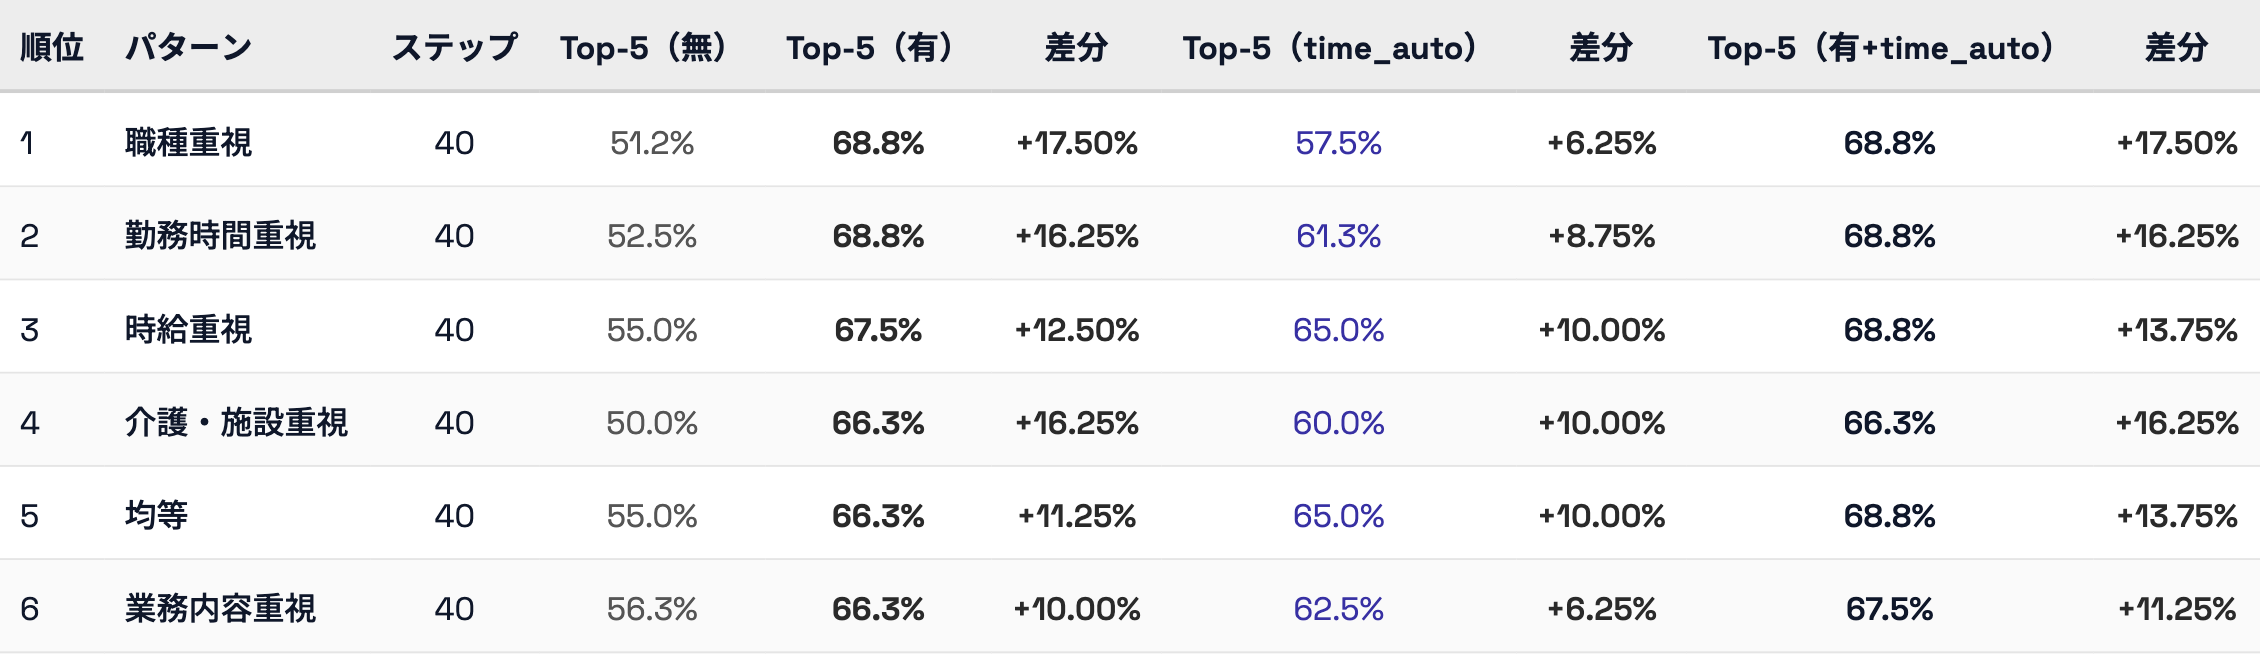
\includegraphics[width=0.9\textwidth]{images/fig1-12.png}
\caption{18名データの重み付けパターン比較（概観）}
\label{fig:20people-patterns}
\end{figure}

\begin{table}[htbp]
\centering
\caption{回避ペナルティ有無の平均精度（18名, \texttt{equal} / 時間重み付け無し / 学習20件）}
\begin{tabular}{l r r r}
\hline
条件 & Top-1 & Top-3 & Top-5 \\
\hline
ペナルティ無し & 0.478 & 0.628 & 0.694 \\
ペナルティ有り & 0.583 & 0.744 & 0.806 \\
差分 & +0.106 & +0.117 & +0.111 \\
\hline
\end{tabular}
\end{table}

\subsubsection*{結果の解釈}
改善幅はTop-3/Top-5で特に大きく、回避ペナルティにより「候補の中身が良くなる（選びやすい候補が残る）」方向に働いたと解釈できる。これは、意味的類似度や条件一致で上位に来ていた求人の中から、回避項目を含むものが順位を下げ、相対的に応募しやすい求人が上位へ移動したためである。

\subsubsection*{考察と限界}
回避業務ペナルティは、ユーザースタディで確認された「避けたい業務」を\textbf{点数に直接反映}できる点で有効である。一方で、(i)タグ付与が不十分な求人（\textbf{該当なし}が多い等）では推定が弱くなる、(ii)回避傾向が弱いワーカーでは差分が小さい、(iii)回避が強いが「例外的に応募したい」状況（報酬が高い、近い等）もあり得る、といった限界もある。今後は、回避度の更新頻度、ペナルティ強度の個別最適化、タグ品質の改善（入力支援や正規化）などが課題となる。

\subsubsection*{時間志向の分布（時間重み自動判別の出力）}
時間重み自動判別は、履歴（過去に選ばれた求人）が\textbf{最近のものに偏っているべきか}、あるいは\textbf{ある程度長い期間を均等に見たほうがよいか}を、履歴の変化の大きさから推定し、内部的に時間重みパターンを切り替える。18名の判定では、\textbf{長期志向が15名、短期志向が3名}であり、多くのワーカーは「好みの中心が大きくは変わっていない」と推定された。

\section{追加実験2：時間志向を同時に扱った場合}
\subsubsection*{目的}
追加実験2では、回避業務ペナルティと、履歴の新しさを考慮する\textbf{時間重み自動判別}を同時に適用したときの挙動を確認する。回避は「仕事内容の好み（避けたい業務）」、時間重みは「好みの変化（最近の履歴を重視すべきか）」に関わるため、両者を同時に入れると互いに強め合う場合もあれば、過剰に絞り込んでしまう場合もあり得る。そこで、同時適用が現実的に有効かを評価する。

\subsubsection*{実装方針とGUI連携}
GUIでは「ペナルティ有無 + 時間重み自動判別 比較」を用意し、\textbf{ペナルティ無し/有り}に加えて\textbf{時間重み自動判別}と\textbf{ペナルティ有り + 時間重み自動判別}を同時に評価できる。

\subsubsection*{長期志向/短期志向の判定（概要）}
時間重み自動判別は、履歴の「好みの中心」が時間とともにどれだけ移動するかを見て、時間重みを切り替える。ここで「中心」とは、求人文を数値にしたベクトル（文章の意味を表す数値列）を平均したものとして扱う。
\begin{itemize}
\item 本研究のデータでは履歴に日付が含まれるため、日付ベースの候補（直近重視の指数減衰、期間制限型）から選択する（期間制限型は直近90日以内を同一重み、それ以前は重み0）。
\item 履歴が十分（8件以上）ある場合、最近ウィンドウ（\texttt{recent\_window = min(5, max(2, n/3))}）とそれ以前の中心を比較し、\textbf{ドリフト（好みの変化量）}を\texttt{1 - cosine(recent\_center, older\_center)}として算出する。ドリフトが0.12未満なら長期志向（好みがあまり変わっていない）と判定し、期間制限型へ切り替える。
\end{itemize}
この判定情報（ラベル、採用パターン、ドリフト、ウィンドウ長）は結果表示に含め、同じワーカーでも「なぜ最近重視になったか/ならなかったか」を追跡できるようにした。

\subsubsection*{時間重みパターンの定義（直近重視の指数減衰 / 期間制限型）}
時間重みは、履歴中の各求人に対して「現在（評価時点）からどれだけ過去か」を表す\textbf{経過日数}に基づいて計算し、履歴求人の埋め込み（意味ベクトル）の\textbf{重み付き平均}としてユーザープロファイルを作るために用いる。実装では、履歴内で最も新しい日付を基準日とし、各履歴求人の経過日数（\texttt{age\_days}）を「基準日 $-$ 当該求人の日付」の日数で定義する。
\begin{itemize}
\item 直近重視の指数減衰：新しい履歴ほど強く重視する方式であり、重みを $w=\left(0.5\right)^{\texttt{age\_days}/7}$ とする（半減期7日）。
\item 期間制限型：直近90日間の履歴のみを重み1、それより古い履歴を重み0として扱う（$\texttt{age\_days}\le 90$なら$w=1$、それ以外は$w=0$）。
\end{itemize}

\subsubsection*{評価視点}
回避ペナルティが有効であることを確認した上で、\textbf{時間志向（長期/短期）の自動判別}を同時に適用した場合の影響を確認する。

\begin{figure}[htbp]
\centering
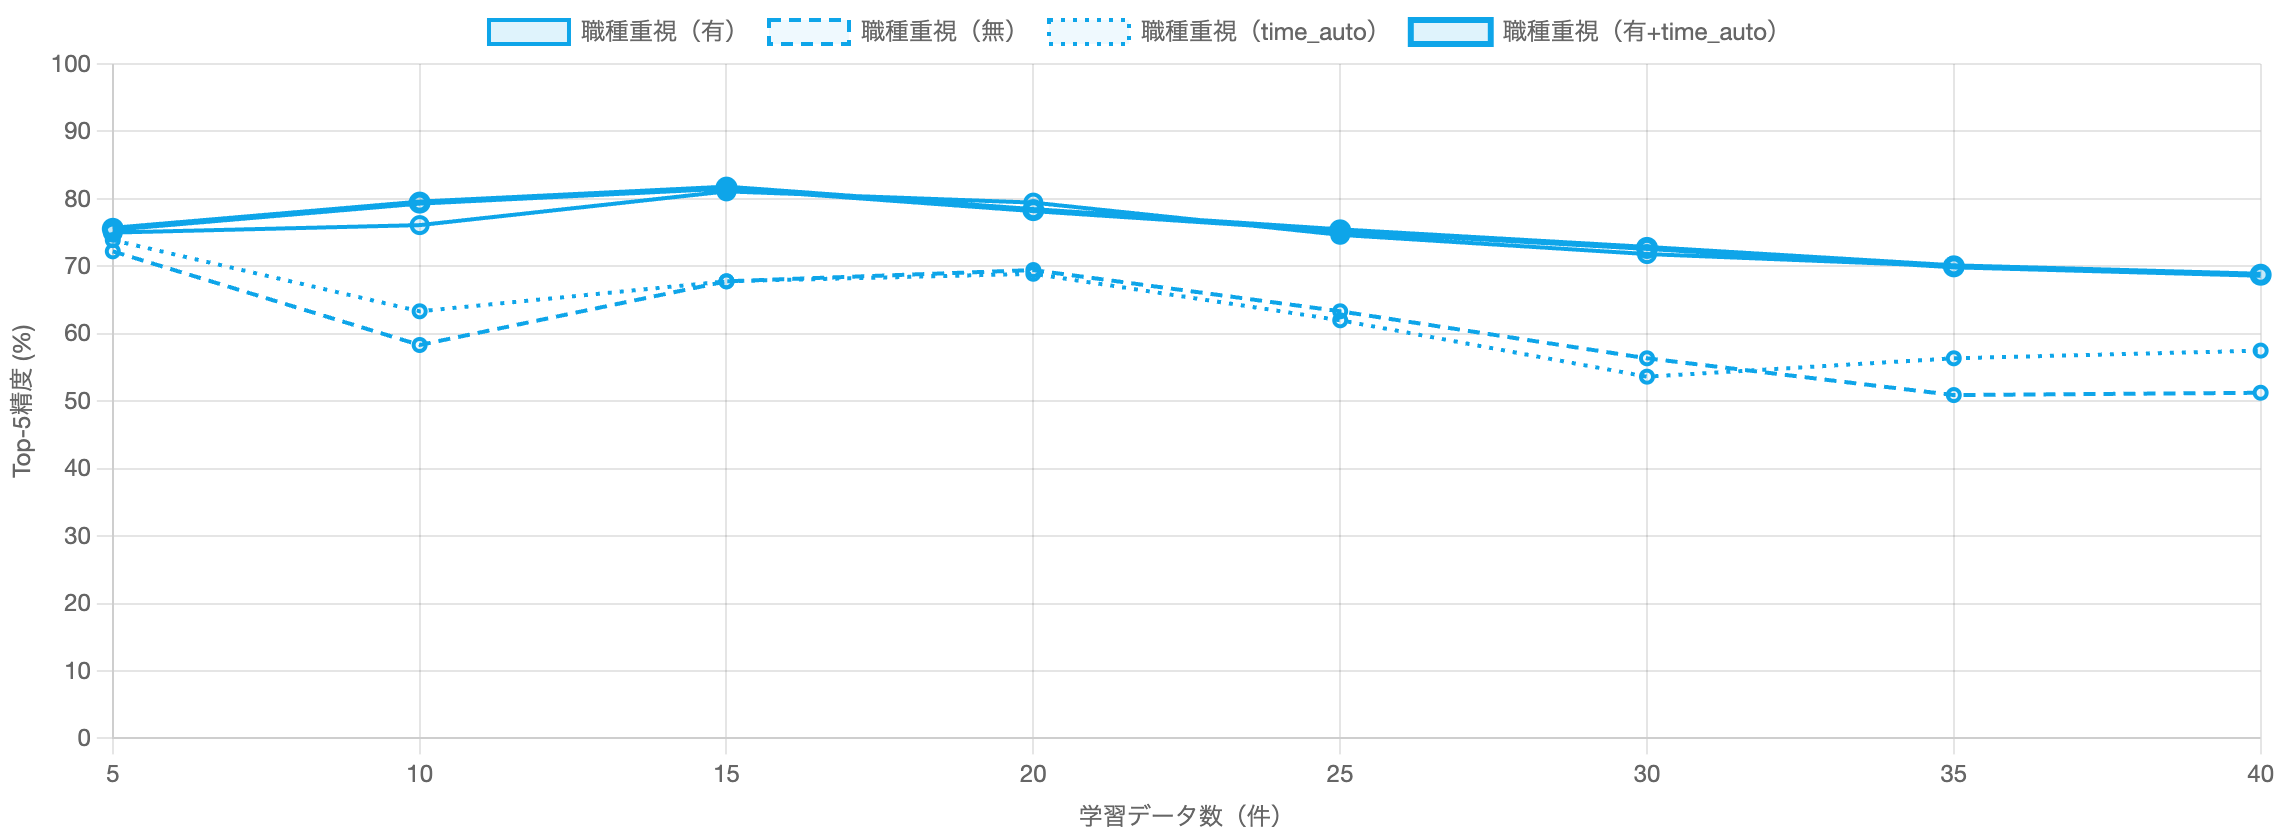
\includegraphics[width=0.9\textwidth]{images/fig1-13.png}
\caption{ペナルティ有無 + 時間重み自動判別の同時評価結果}
\label{fig:penalty-and-auto-time}
\end{figure}

\subsubsection*{結果（4条件の同時比較）}
同時比較では、(A)ペナルティ無し、(B)ペナルティ有り、(C)時間重み自動判別、(D)時間重み自動判別+\textbf{ペナルティ有り}の4条件を、同じワーカー・同じ手順で評価した。10名データでは、\textbf{(D)がTop-1/Top-3/Top-5で最も高い平均値}となり、時間重み自動判別と回避ペナルティが競合せず補完的に働くケースが多いことを示した。

% 表7.2（10名データの4条件比較）は本文から除外する
\iffalse
\begin{table}[htbp]
\centering
\caption{4条件同時比較の平均精度（10名, \texttt{equal}）}
\begin{tabular}{l r r r}
\hline
条件 & Top-1 & Top-3 & Top-5 \\
\hline
(A) ペナルティ無し & 0.399 & 0.505 & 0.580 \\
(B) ペナルティ有り & 0.480 & 0.637 & 0.697 \\
(C) 時間重み自動判別 & 0.433 & 0.533 & 0.612 \\
(D) 時間重み自動判別 + ペナルティ有り & 0.487 & 0.641 & 0.707 \\
\hline
\end{tabular}
\end{table}
\fi

\begin{table}[htbp]
\centering
\caption{4条件同時比較の平均精度（学習20件, 18名, \texttt{equal}）}
\label{tab:avoidance-timeauto-20workers-equal}
\begin{tabular}{l r r r}
\hline
条件 & Top-1 & Top-3 & Top-5 \\
\hline
(A) ペナルティ無し & 0.478 & 0.628 & 0.694 \\
(B) ペナルティ有り & 0.583 & 0.744 & 0.806 \\
(C) 時間重み自動判別 & 0.494 & 0.650 & 0.706 \\
(D) 時間重み自動判別 + ペナルティ有り & 0.567 & 0.750 & 0.794 \\
\hline
\end{tabular}

\end{table}

\begin{table}[htbp]
\centering
\caption{4条件同時比較の平均精度（学習15件, 18名, \texttt{equal}）}
\label{tab:avoidance-timeauto-20workers-equal-step15}
\begin{tabular}{l r r r}
\hline
条件 & Top-1 & Top-3 & Top-5 \\
\hline
(A) ペナルティ無し & 0.517 & 0.600 & 0.678 \\
(B) ペナルティ有り & 0.600 & 0.717 & 0.789 \\
(C) 時間重み自動判別 & 0.517 & 0.611 & 0.694 \\
(D) 時間重み自動判別 + ペナルティ有り & 0.611 & 0.717 & 0.783 \\
(E) 7日半減（指数減衰）+ ペナルティ有り & 0.584 & 0.716 & 0.784 \\
\hline
\end{tabular}

\end{table}

\subsubsection*{結果と考察}
図\ref{fig:penalty-and-auto-time}に示す通り、\textbf{回避ペナルティの有無}と\textbf{時間重み自動判別の選択結果}を同時に可視化することで、長期志向/短期志向の違いと上位候補の入れ替わりを把握できるようになった。個別ワーカーでは、ペナルティ付与により「避けたい業務」を含む求人が上位から外れるケースが見られ、時間重み自動判別を併用した場合にも同様の傾向が確認された。

一方で、平均精度の増減はワーカーの履歴量や回避傾向の強さに依存する。今後は\textbf{回避度の更新頻度}や\textbf{ペナルティ強度の個別最適化}（例：回避が強い人ほど $w$ を上げる、回避が弱い人は $w$ を下げる）を検討する必要がある。また、回避項目の推定は「候補に出たのに選ばれない」を根拠にするため、候補生成の偏り（特定タグが候補に出にくい等）がある場合には推定が難しくなる。実運用で導入する際は、候補生成・表示・選択のログ設計も含め、推定が安定するデータ収集が重要である。
